\Chapter{Kínai karakterek felismerése}

\begin{comment}{Be kellene majd hivatkozni, hogy az említett dolgok hol találhatók meg a szakirodalomban (pl.: kínai tankönyvek)}
\end{comment}

\begin{comment}{Itt a következő mire vonatkozik?}
\end{comment}

\section{Az alapvonások}

Az írásjegyek felépítésének következő lényeges szabálya az írásjegy vonásainak sorrendje. Az írásjegyek – bármilyen bonyolult legyen is némelyik – tulajdonképpen néhány igen egyszerű vonalból épülnek fel. Ezek az írásjegyek alapelemei, vagy alap-ecsetvonásai. \Aref{fig:alapvonasok}. ábrán az alapvonások néhány főbb típusa látható. Természetesen az alapvonásoknak több változata is lehetséges (méret, vastagság, irány) attól függően, hogy az írásjegy melyik részén helyezkedik el.

\begin{figure}
	\centering
	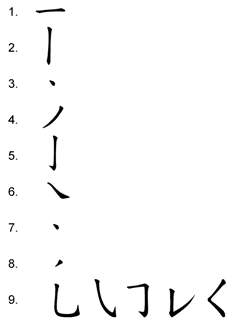
\includegraphics[scale=0.5]{chinese_strokes}
	\caption{A kínai karakterek alapvonásai}
	\label{fig:alapvonasok}
\end{figure}

Minden egyes vonásnak megvan a felépítési szabálya: az ecsetvonásoknak meghatározott sorrendben kell követniük egymást, még pedig általános elvként az írásjegyek határait alkotó virtuális négyszög bal felső sarkából lefelé és jobbra haladva. Az írásjegy gerincét, fő szerkezeti elemét adó nagyobb vonást, ha az egész írásjegyet átjárja, legutoljára húzzák.

\section{A vonássorrend szabályai}

Az előző szakaszban említett általános elv mellett az alábbi szabályokat alkalmazhatjuk az írásjegyek vonásainak sorrendjének meghatározásához.
\begin{enumerate}
	\item A vízszintes vonások megelőzik a függőleges vonásokat.
	\item A balra lejtő vonások megelőzik a jobbra lejtő vonásokat. 
	\item Az írásjegyek írását felülről kell kezdeni. 
	\item Az írásjegyet balról jobbra haladva építik fel. 
	\item A felülről keretezett írásjegyeknél előbb a keretet kell meghúzni. 
	\item Az alulról keretezett írásjegyeknél a keretet legvégül kell meghúzni. 
	\item A teljes keretet mindig legvégül kell bezárni.
\end{enumerate}

Egy szimmetrikus felépítésű írásjegynél előbb a középső részt kell kialakítani, s csak azután az oldalakat. Erre láthatunk egy példát \aref{fig:sorrend_pelda}. ábrán.

\begin{figure}
	\centering
	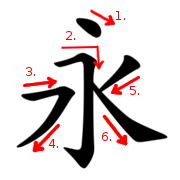
\includegraphics[scale=1.0]{images/vonasrend_ordered.png}
	\caption{Példa egy szimmetrikus írásjel vonásainak sorrendjére}
	\label{fig:sorrend_pelda}
\end{figure}

A kínai írásjegyek különböző számú alapvonásokból épülhetnek fel. Ezek közül a legegyszerűbb a csupán egyetlen vízszintes vonalból álló „egy” jelentésű \begin{CJK*}{UTF8}{gbsn}
一
\end{CJK*} ji írásjegy. A kínai írásrendszer más, egy vonásból álló írásjegyet nem tartalmaz. Aránylag ritkák a két vonásból álló írásjegyek is, például: \begin{CJK*}{UTF8}{gbsn}
二
\end{CJK*} er„kettő”,
\begin{CJK*}{UTF8}{gbsn}
十
\end{CJK*} si „tíz”,
\begin{CJK*}{UTF8}{gbsn}
人
\end{CJK*} zsen „ember” stb. A hagyományos írásjegyek zöme 15–30 vonásból épül fel (átlagosan 9 vonásból). Esetenként azonban ennél jóval több vonásból álló írásjegyek is előfordulhatnak, melyek tulajdonképpen már több önálló írásjegy összevonásának is tekinthetők. Ritkák ugyan, de léteznek 50 vagy akár 80 vonásból álló írásjegyek is.

\begin{comment}{Ha a vonások számát valahol táblázatos formában el lehet érni, akkor érdemes ide egy hisztogramot is berakni.}
\end{comment}

\section{OCR megvalósítások}

\subsection{Az optikai karakterfelismerés feladata}

A különböző formátumú dokumentumok kezelésének egyik speciális esete, amikor a kezelendő dokumentumok még nem állnak rendelkezésre elektronikus formában. Ebben az esetben szinte mindig arról van szó, hogy a dokumentumok kinyomtatva, papír alapú hordozón jelennek meg. A későbbi feldolgozáshoz értelemszerűen digitalizálni kell a még nem digitalizált, papíron, nyomtatásban vagy írásban meglévő dokumentumokat, hogy az után elektronikusan szerkeszthető és feldolgozható legyen. Ebben a szituációban kap szerepet az optikai karakterfelismerés (\textit{Optical Character Recognition}, OCR). Az optikai karakterfelismerés a mesterséges intelligencia jelfeldolgozó és generalizációs képességeit kiaknázva képes nyomtatott, papír alapú dokumentumokon lévő karaktereket felismerni.

Az alap probléma itt az, hogy a nyomtatott, papír alapú dokumentumok esetében nagy zajaránnyal kell megküzdeni annak érdekében, hogy a releváns információt kinyerjük az érzékelt képi jelek és minták közül. Nyomtatott dokumentum esetében ilyen zajnak tekinthető például egy apró folt a papíron, tintaelmosódás, tintahiány, homályos háttér, apró gyűrődés a papíron, túl közeli vagy egybeolvadó betűk, betű dőlésszögének ingadozása stb. Kézírás esetén a kihívás még nagyobb, hiszen itt a személyiségjegyek sokszínűségéből adódó írásminták kavalkádjából kell megkűzdeni, hogy fel tudjuk imsertetni a karaktereket. Mind a nyomtatott, mind pedig a kézírásos esetben az optikai karakterfelismerő rendszer egy tanulási fázist követően képes olyan mintákat is osztályozni (a megfelelő karaktert felismerni), amelyekkel a tanulási fázisban nem találkozott, tehát megvan a szükséges generalizációs képessége.

Vannak készen elérhető OCR megolások, amelyek tipikusan az alábbi két részből állnak.
\begin{enumerate}
\item A szkennelő fejből, amely a dokumentum egészét vagy részeit beszkenneli. Hardverről van szó, ami elvégezi a digitalizálást. Két fizikai jelenségen alapszik fényvisszaverődésen és a fényelnyelésen.
\item  A mesterséges intelligencia szoftverből, ami elvégezi a beérkezett minták osztályozását, azaz magát a karakterfelismerést.
\end{enumerate}

\begin{comment}{Hivatkozni kellene konkrét ilyen eszközöket}
\end{comment}

\begin{figure}[h]
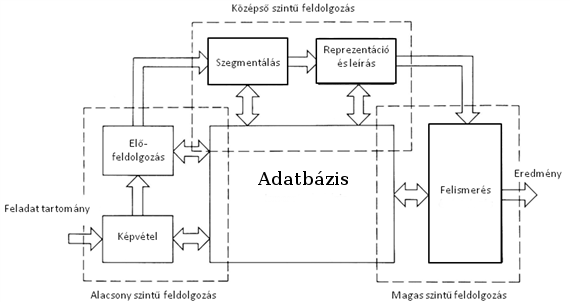
\includegraphics[scale=0.65]{ocr}
\centering
\caption{Az OCR-es feldolgozás szintjei}
\label{fig:feldolgozasi_szintek}
\end{figure}

Az OCR-el való feldolgozás során alapvetően három szintet különböztethetünk meg (\ref{fig:feldolgozasi_szintek}. ábra).

\begin{enumerate}
\item Alacsony szintű (\textit{low-level}) feldolgozás
	\begin{itemize}
	\item A bemenet egy zajos kép, a kimenet pedig már egy tisztított, későbbi feldolgozásra alkalmasabb kép.
	\item Itt a kép minőségének a javításához az elterjedt képfeldolgozási előfeldolgozó algoritmusokat használják.
	\item Jellemző előfeldolgozások: \textit{zajszűrés, élesítés, finomítás, világosítás, maszkolás}.
	\end{itemize}
\item Középső szintű (\textit{intermediate-level}) feldolgozás
	\begin{itemize}
	\item A bemenetek képek, de a kiementek már a képekből nyert jellemzők.
	\item A kép komponenseinek kiemelése (szegmentálás) és azok jellemzése.
	\item Bizonyos mértékű mesterséges intelligencia/gépi tanulás szükséges hozzá.
	\end{itemize}
\item Magas szintű (\textit{high-level}) feldolgozás
	\begin{itemize}
	\item A felismert objektumok együttesének érzékelése (osztályozási probléma).
	\item Felismerés és értelmezés (interpretáció).
	\item Ezen a szinten kap kiemelt szerepet a mesterséges intelligencia módszereinek alkalmazása.
	\end{itemize}
\end{enumerate}

Az adatok kezelését struktúrált, ellenőrzött formában érdemes megoldani, amihez úgy általában egy adatbázis szükséges.

\begin{comment}{Ez a felsorolás így elég vázlatos. Részletezni, vagy legalábbis teljes mondatokra át kellene írni őket.}
\end{comment}

\begin{itemize}
\item A felismerni kivánt képek halmaza. A képekhez címkék tartoznak, ami szükséges a mesterséges intelligencia tanulás során.
\item A feldolgozott képek
	\begin{itemize}
	\item visszakerülnek az adatbázisba vagy
	\item továbbítják azt egy magasabb szintre
	\end{itemize}	  
\item Az interneten rengeteg adatbázis található: \textit{mnist, imagenet, kaggle, CASIA}
\item !Kiegészíthető! Az adatok előkészítése:
	\begin{enumerate}
	\item Kiválasztás, feldolgozás, transzformálás
	\item Publikus adatbázis vagy saját adatbázis
	\item Konvertálás vektorra a gépi feldolgozás érdekébe
	\end{enumerate}
\end{itemize}

\cite{feldolgozasi_szintek}

\begin{comment}{Érdemes konkretizálni az adatbázis és a nyilak jelentését, hogy ne legyen annyira általános!}
\end{comment}

\subsection{Szegmentációs módszerek}

\begin{comment}{A szegmentálást úgy általában is használják kéfeldolgozásnál a régiók elkülönítéséhez. Ki kellene hangsúlyozni, hogy mi a kettő között a különbség.}
\end{comment}

A szegmentáció során a karakterek közötti éles határ megtalálása a cél annak érdekében, hogy téves minták ne kerüljenek osztályozásra (például két fél karakter). A szegmentáció feladata lehet az is, hogy a karakter-dőlésszögeket, karakterméreteket normalizálja. Sok esetben a szöveges dokumentumokban nem csak karakterek vannak, hanem képek és egyéb, a felismerés szempontjából nem lényeges szimbólumok. A szegmentáció további feladata tehát az is, hogy az ilyen, számunkra nem releváns grafikus objektumok közül kiszűrje a csak karaktereket tartalmazó szöveges részeket. \Aref{fig:ocr_segmentation}. ábrán láthatunk egy példát arra, hogy hogyan képes az algoritmus kiemelni az egy karakterhez tartozó képrészt.

\begin{figure}
\centering
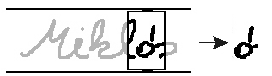
\includegraphics[scale=1.0]{ocr_segmentation}
\caption{Példa egy név karaktereinek a szegmentálására}
\label{fig:ocr_segmentation}
\end{figure}

\begin{comment}{Ez itt saját kép?}
\end{comment}

\subsection{Optikai előfeldolgozás}

Az előfeldolgozás a bemeneti minta komplexitásának csökkentésére szolgál, és annak legjellemzőbb vonásait emeli ki. Különösen nagy jelentősége van a kézírás felismerésekor, ugyanis az írott betűk jóval komplexebb mintákat alkothatnak, mint a nyomtatott betűk. A jellemzők kiemelése során a komplexitás úgy csökken, hogy közben a legjellemzőbb információk megmaradnak és ezáltal a későbbi feldolgozás számításigényét redukálhatjuk. Ez a folyamat tulajdonképpen egy komplexitáscsökkentéssel járó digitalizáció. \Aref{fig:ocr_preprocess}. ábra egy egyszerű digitalizálási módszert mutat, amikor az analóg jelre egy mátrixot reprezentáló rácshálót illesztünk, és amelyik cellán átmegy az analóg karakter, az az elem a mátrixban 1 értéket vesz fel (fekete), egyéb esetben pedig 0-t (fehér).

\begin{figure}
\centering
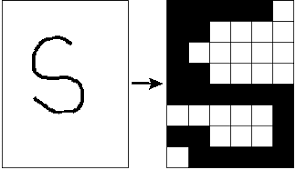
\includegraphics[scale=0.65]{ocr_preprocess}
\caption{Jellemzők kinyerésének egy fázisa, amely a dimenzió csökkenésével jár}
\label{fig:ocr_preprocess}
\end{figure}

\begin{comment}{Meg kellene említeni a dimenziók csökkentését is, mert az átalakítás során a komplexitás olyan formában csökken, hogy a dimenzió csökken és információ vész el.}
\end{comment}

\subsection{Felismerés}

Az osztályozás során történik meg a tényleges karakterfelismerés. A karakterfelismerő módszer a bemeneti jellemzővektor alapján dönti el, hogy az ismert karakterek közül melyikre hasonlít a legjobban a bemeneti vektor. Így a karakterfelismerési probléma egy asszociatív memóriát igénylő feladat, amelynek során a tárolt memóriaelemek közül kell előhívni azt, amely a bemeneti mintának legjobban megfelel.\\

\subsection{Kínai karakter felismerés}

\begin{comment}{Itt ez nagyon általánosan kezdődik. Vagy az alcímet érdemes megváltoztatni, vagy egyből a lényegi részre térni rá a kínai karakterek felismerésével kapcsolatban.}
\end{comment}

A számítógépek képesek felismerni a karaktereket, beszélik és megértik az emberi nyelveket, kommunikálnak az emberi nyelven egyre elterjedtebb számítógépes iparban. Karakterfelismerés óriási időt takaríthat meg az adatok és üzenetek számítógépekbe történő írásához. Azonban, a kínai karakterek felismerése a számítógépen sokkal nagyobb kihívást jelent, mint a többi nyelveknél, mert hatalmas mennyiségű karakterkészlettel rendelkezik (27484 karakter).

A karakterek felismerése lehet online és offline karakterfelismerés. A fő különbség az, hogy az online karakterfelismerés rögzíti az ecsetvonások mozgását, míg az offline karakterfelismerés pusztán a karakter geometriai alakján alapul.

Az online karakterfelismerés során lehetőségünk van zaj generálására. Az ecsetvonások mozgása során véletlenszerű zajokat adhatunk hozzá. A zajos képekkel való betanítás a rendszerünk robusztusságát éri el.

Zaj hozzáadás:
\begin{itemize}
\item Pontszerű zajok: véletlenszerű fekete pixeltartomány hozzáadása
\item Elmosódások: Gauss elmosás alkalmazása
\item Forgatás: affin, perspektív transzformáció vagy forgatás origó körül 
\item Alacsony kontraszt: pixel megfelelő értékeinek szorzása
\end{itemize}

\begin{center}
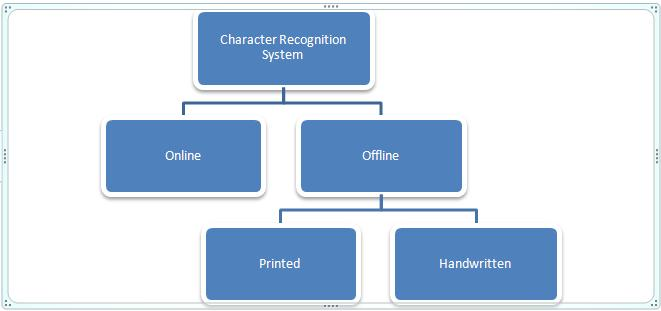
\includegraphics[scale=0.75]{ocr_online_offline}
\end{center}

Az OCR folyamatba bevitt képek általában a szkennerekből származnak, amik képet és karaktert tartalmaznak. A karakterek gyakran különböző méretűek és betűtípusokat.

\begin{comment}{Az online és offline felismerés megkülönböztetése kapcsán érdemes említeni, hogy a zaj generálásánál az online jelleg figyelembe vételre kerül majd.}
\end{comment}

Az előfeldolgozás során a következők jöhetnek szóba: 
\begin{itemize}
\item karakterek szétosztása a bemenetek függvényébe
\item a zaj megszüntetése
\item normalizálni a betűméretet és pozícionálni a filtert (kernel-t)
\item stroke váz generálása (thinning)
\end{itemize}

\begin{comment}{Legalább 3-4 hivatkozás kellene ezekhez a részekhez.}
\end{comment}

A jellemző alapú módszerek kivonják a karakter jellemzőit, mivel ezek a jellemzők matematikailag számítottak, amire alkalmas számítógép. Így az optikai karakterfelismerés (OCR) nem igazán az optikai alapokon nyugszik, hanem inkább a matematikai számításokhoz köthető.

\begin{comment}{A stroke szavak használata is jó, csak akkor érdemes valahol megadni, hogy az alapvonásokkal mi a viszonya.}
\end{comment}

Amint említettem, minden kínai karakternek egyedi geometriai alakja van, amiket a stroke-ok alakítják. A kínai karakterek felismerésének alapja a stroke-ok és a strukturális jellemzők. Hosszú ideig ez a módszer befolyásolta a kínai karakterfelismerés kutatási irányát.
A karakter struktúrális lebontására láthatunk egy példát \aref{fig:ocr_features}. ábrán.

\begin{figure}
\centering
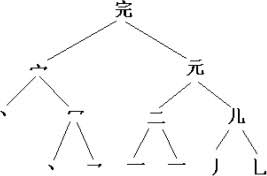
\includegraphics[scale=0.8]{ocr_features}
\caption{Egy kínai karakter lebontása alapelemekre, hogy az után azokat, mint jellemzőket lehessen használni}
\label{fig:ocr_features}
\end{figure}

Azonban ez nagyon nehéz a gyakorlatban, mert a stroke és a struktúrák közötti kapcsolat nagyon instabil. A stroke-ok és a strukturális jellemzők nem tudják hatékonyan kivonni a jellemzőket vagy nem praktikus.

Rengeteg mód van a jellemzők kivonására, például lehet alapozni az él detektálásra, transzformációkra, rács jellemzőkre, kulcsfontosságú jellemzőkre, vektor vonali jellemzőkre.

Miután rendelkezésre állnak a módszerek, amikkel ki lehet nyerni a jellemzőket, hozzáfoghatunk a végleges kimenet előállítására. Lehetséges, hogy különböző felismerési rendszereket állíthat össze és összehasonlíthatjuk a kimeneteket. Azonban ez extra számítási költséget igényel, viszont a pontosság tovább javítható.

Mikor a felismerési rendszer kimenetet generál, lehetséges, hogy néhány karaktert tévesen osztályoz. Ez javítható a különböző bemeneti minták növelésével.

\begin{comment}{A leírás alapján itt még nem áll össze, hogy ez még az irodalmi áttekintés, vagy már a saját módszernek a bemutatása.}
\end{comment}

\subsection{Implementálás}

\begin{comment}{A betűtípusokra részletesebben ki kellene térni. Irodalmi hivatkozás itt is mindenképpen kell majd.}
\end{comment}

Egy olyan algoritmust mutatok be, ami képes kínai karakterek felismerésére sok különböző betűtípussal (pl. Song, Fang, Kai, Hei, Yuan, Lishu, Weibei és Xingkai). Ezekre a betűtípusokra \aref{fig:chenese_fonts}. ábrán láthatunk néhány példát.

Az algoritmus származtatott jellemzőkön alapul, és egy szótár halmazt használ. Először egy 3 szintes illesztést végez mindegyik szótárhoz képest. Az ilyen illesztésekhez kapcsolódó távolsági méréseket ezután egy központi diszkriminátorba táplálják, hogy a végső felismerési eredményt kiadják. Gyors és a pontos felismerést ért el mind a címben az összes 8 betűtípust és mind a főoldalon, amelyhez az első 4 általánosan használt betűtípus tartozik.

\begin{figure}
\centering
\begin{tabular}{ c c }
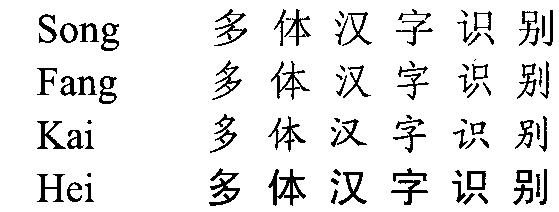
\includegraphics[scale=0.35]{chinese_fonts1} & 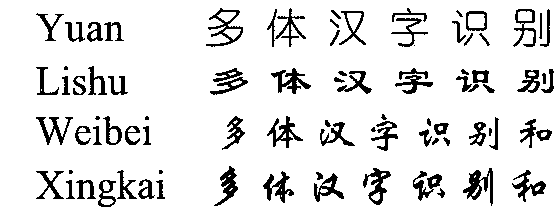
\includegraphics[scale=0.35]{chinese_fonts2}
\end{tabular}
\caption{Különféle kínai betűtípusok}
\label{fig:chinese_fonts}
\end{figure}

A funkciókivonás fontos eleme az OCR-nek. Az algoritmus egy 8-dimenziós vektor tartozik $[d_1, d_2, \ldots d_8]$. Kiszámítása az alábbi összefüggés segítségével történik
$$
d_i = \dfrac{l_i}{\sqrt{\displaystyle \sum_{k=1}^8 l_k^2}},
$$
ahol $i = 1, \ldots, 8$, és $l_i$ a csatlakoztatott fekete képpontok száma $i$-edik irányban. Erre egy példát láthatunk \aref{fig:8direction}. ábrán.

\begin{figure}
\centering
\begin{tabular}{ c c }
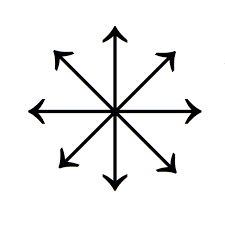
\includegraphics[scale=0.6]{8direction} & 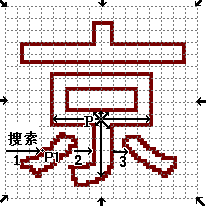
\includegraphics[scale=0.6]{ocr_PDC}
\end{tabular}
\caption{A jellemző irányok használati módja a karakterfelismerés során}
\label{fig:8direction}
\end{figure}

Az OCR rendszereknél, a felismerési algoritmusok két szakaszból állnak: tanítás és tesztelés. A hálózat súlyait a képzés során határozzák meg. A képzés után a rendszer átkapcsol a tesztelési fázisra, és a szótárak szerint meghatározza a legvalószínűbb karakterindexet.

A hierarchikus illeszkedés három szintből áll. Az első szint egy osztályozó, ami felhasználja a transzformált jellemzőket. Ezután a jellemzőket egy második szintű osztályozónak adják át. Az osztályozó több elemet is kiemel (kisebb számú kimenet). A harmadik szint az összes elemet használni fogja, a karaktert a végső felismerés eredményeként kiválasztja.

A 3 szintű hierarchikus struktúra nem csak csökkenti a számítási komplexitást, hanem figyelembe veszi a jellemzők összetevőit. Az utóbbi növeli felismerési pontosság. A 3-szintű struktúra hatékonysága a felismerési arány, a sebesség és a memória használat.

Minden tesztet két kínai mintán végzik, összesen 7510 karakterrel. Ezek az eredmények azt mutatják, hogy a 8 betűtípus átlagos felismerési aránya 99,32\% a képzési minták esetében, pedig 98,96\%. A betűtípusonként eredményeket \aref{tab:ccr_results}. táblázat foglalja össze.

\begin{table}
\centering
\begin{tabular}{ |c|c|c|c|c|c|c|c|c|c|}
\hline
Font & Song & Fang & Kai & Hei & Yuan & Lishu & Weibei & Xingkai & Average\\
\hline
Train & 99.82 & 99.64 & 99.81 & 99.57 & 98.77 & 98.75 & 99.35 & 98.82 & 99.32\\
\hline
Test & 99.71 & 99.50 & 99.80 & 99.09 & 98.43 & 98.15 & 98.78 & 98.19 & 98.96\\
\hline
\end{tabular}
\caption{Az elérhető karakterfelismerő rendszer hatékonysága különböző betűtípusok esetén}
\label{tab:ccr_results}
\end{table}

A kísérleti eredmények azt mutatják, hogy a javasolt algoritmus képes gyorsan és pontosan felismerni a karaktereket akár 8 különböző betűtípussal is. Az algoritmus kiváló felismerési teljesítményt nyújt a 4 leggyakrabban használt betűtípusnál \cite{ccr}.


!Kiegészíteni lehet CCR HANDWIRTTEN CHAR!
